\documentclass{article}
\usepackage{graphicx} % Required for inserting images
\usepackage{float}

\title{Relazione Progetto Programmazione ad Oggetti}
\author{Marco Cola}
\date{}
\begin{document}

\maketitle

\begin{tabbing}
    Oggetto: \= Relazione progetto Programmazione ad Oggetti \\
    Studente:  \=  Marco Cola, mat.2079237 \\
    Titolo: \= Sensor Simulation \\
    \\
\end{tabbing}

\section{Introduzione}
Sensor Simulation è un generatore casuale di valori per sensori di tre tipologie differenti,
Temperatura, Umidità e Polveri Sottili. Ogni sensore ha un unità di misura differente, ho scelto i
Celsius (°C) per i sensori di Temperatura, la percentuale (\%) per i sensori di Umidità e la
concentrazione media di PM10 nell’aria calcolata in µg/m³ per le Polveri Sottili. La simulazione
permette le seguenti operazioni su un Sensore: la creazione, ovvero l’aggiunta di un nuovo sensore
alla lista, la modifica del nome, la rimozione dalla lista dei sensori creati e la ricerca all’interno di
questa lista tramite searchbar.
L’applicazione permette inoltre l’avvio di una simulazione per ognuno dei tre tipi di Sensori,
generando valori casuali calcolati in un arco temporale di 7 giorni, mostrando le informazioni per
ogni sensore del grafico selezionato, rappresentato da un punto rosso. Infine la simulazione permette il salvataggio della corrente simulazione in un file di testo mediante la funzione “Save” del menu a tendina File (“Ctrl+S”), che potrà poi essere riaperto in seguito mediante la funzione “Open” (“Ctrl+O”), per rispettare la permanenza dei dati dei sensori generati.
La scrittura del codice ed i commenti ai vari metodi e alle classi è in lingua inglese per aderire allo
standard internazionale e lasciare aperta la possibilità di collaborazione nell’ambiente dello
sviluppo software globale.

\section{Descrizione del Modello}
Il progetto segue il pattern architetturale MVC (Model View Controller) per separare nettamente la parte di View da quella di Modello, permettendo il riutilizzo del codice C++ della parte di Modello in caso si voglia sviluppare l’applicazione con un framework differente da Qt. La parte di Controller è rappresentata da una classe SensorManager, che fa “da tramite” tra le due.
Il Modello logico è composto da una classe base Sensor astratta, dalla quale derivano tre classi concrete: Temperature, Humidity e Dust. 
La classe base astratta Sensor rappresenta le informazioni comuni a tutti i sensori, ovvero nome e ID, per i quali sono implementati opportunamente metodi getter e setter. Per ognuna delle sottoclassi concrete di Sensor è implementato un metodo calculateValue, responsabile del calcolo del valore casuale per la tipologia di Sensore della classe, il metodo utilizza un generatore di numeri casuali non deterministico \verb|std::random_device rd;| il quale tramite un generatore di numeri casuali basato sull’algoritmo Mersenne Twister 
\verb|std::mt19937 gen(rd());| genera un valore casuale nei limiti definiti dalla singola implementazione. 
La classe concreta Temperature rappresenta un sensore di Temperatura in gradi Celsius.  
La classe concreta Humidity rappresenta un sensore di Umidità in percentuale.
La classe concreta Dust rappresenta un sensore di Polveri sottili in µg/m³.


\begin{figure}[h]
    \centering
    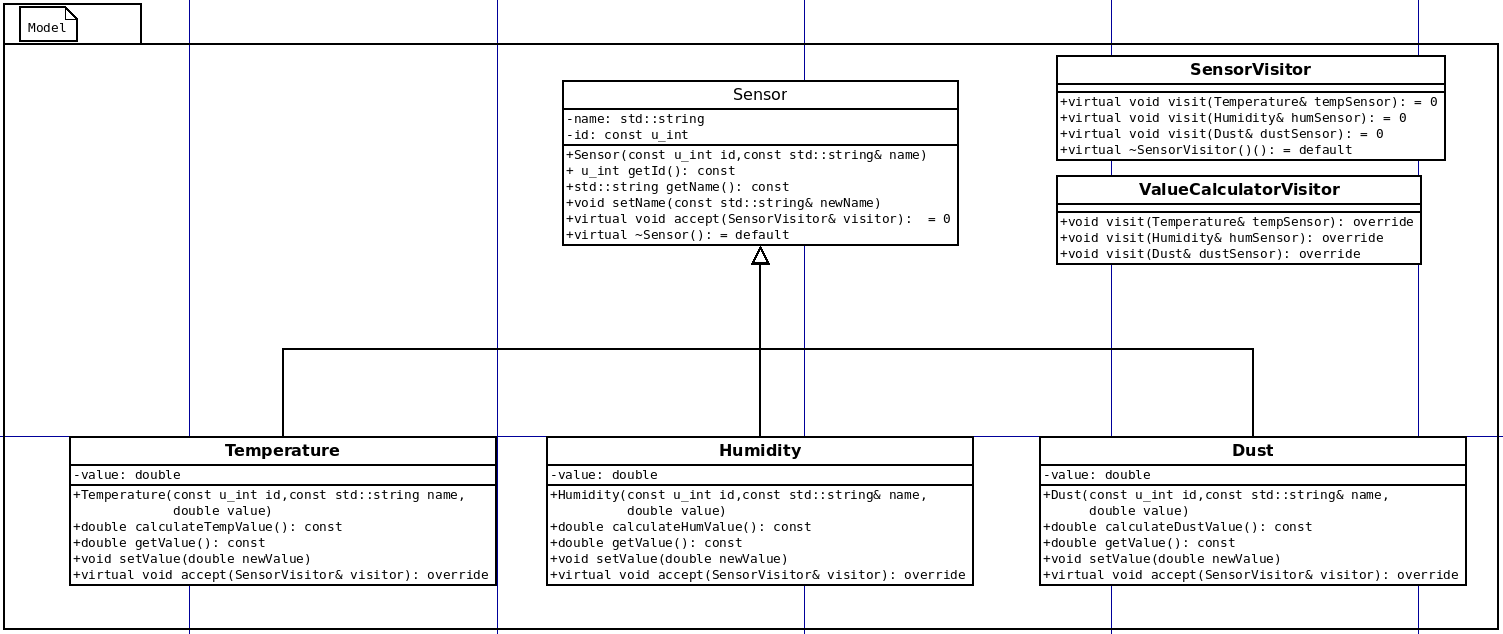
\includegraphics[width=\textwidth]{Logica.png}
    \caption{Parte di Modello}
    \label{fig:Parte di Modello}
\end{figure}


Poiché le classi del modello si comportano come dei Data Transfer Object (DTO) e non espongono alcuna funzionalità rilevante, si è scelto di utilizzare il design pattern Visitor per consentire di estendere il comportamento delle classi di sensori senza modificarne il codice. A tal fine sono state realizzate le classi astratte SensorVisitor e ValueCalculatorVisitor. La classe  SensorVisitor è una classe base astratta che definisce un'interfaccia per le operazioni che possono essere eseguite su vari tipi di sensori. La sua presenza permette di aggiungere nuove operazioni ai sensori senza dover modificare le classi dei sensori stessi. La classe ValueCalculatorVisitor è una concreta implementazione di SensorVisitor che esegue una specifica operazione: calcola e aggiorna il valore di ciascun sensore, in questo modo la logica di calcolo dei valori viene centralizzata in una singola classe, facilitando la manutenzione e l’estensione.

La parte di Controller, viene affidata alla classe SensorManager, che ha il compito di gestire gli input dell’utente che arrivano dalla MainWindow e restituire i valori calcolati e le informazioni richieste dalla parte di Modello. 

La responsabilità principale della classe SensorManager è quella di gestire la creazione, l'aggiornamento, l’aggiunta, la rimozione, la modifica e la ricerca dei sensori tramite ID oppure Nome, mantenendo un elenco di sensori tramite un vector e fornendo metodi per interagire con questi sensori. I sensori vengono memorizzati in un vettore che contiene puntatori unici a oggetti ‘Sensor’, l'uso di \verb|std::unique_ptr| garantisce che ogni sensore sia gestito da un solo puntatore, prevenendo problemi di gestione della memoria.

\begin{figure}[h]
    \centering
    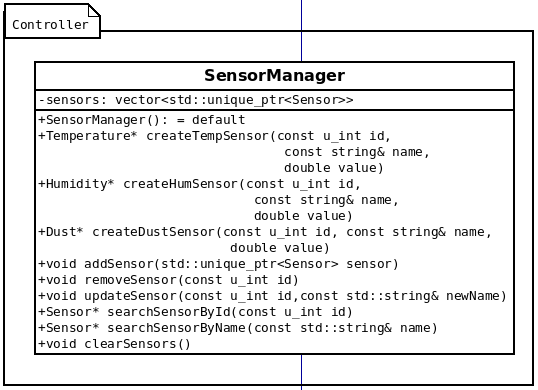
\includegraphics[width=0.5\textwidth]{Controller.png}
    \caption{Parte di Controller}
    \label{fig:Parte di Controller}
\end{figure}

Infine la parte di View, ovvero l’interfaccia grafica che viene presentata all’utente, è composta in questo modo:

La classe principale MainWindow contiene tutti i Widget con cui l’utente può interagire o solo visualizzare. I principali sono: SearchBar, per la ricerca dei sensori nella lista, SensorCharts per la rappresentazione grafica di una serie di valori tramite QtCharts, SensorInfo che mostra i valori del sensore selezionato nella lista di sensori creati o quelli del sensore selezionato nel grafico ed infine SensorCreateDialog, finestra di dialogo che si apre quando si seleziona il QPushButton “Add”, che permette all’utente di assegnare un nome e il tipo al sensore che sta creando.  Altri widget che vengono creati direttamente nella MainWindow sono: la barra del menu, contenente un menu a tendina File che permette il salvataggio e l’upload della configurazione corrente, un tasto Modify, che se premuto dopo la selezione di un sensore dalla lista permette di modificarne il nome tramite una finestra di dialogo ed infine nella classe MainWindow è presente un QcomboBox SelectSimulation, che consente all’utente di selezionare il tipo del sensore per la simulazione nel grafico.

\begin{figure}[H]
    \centering
    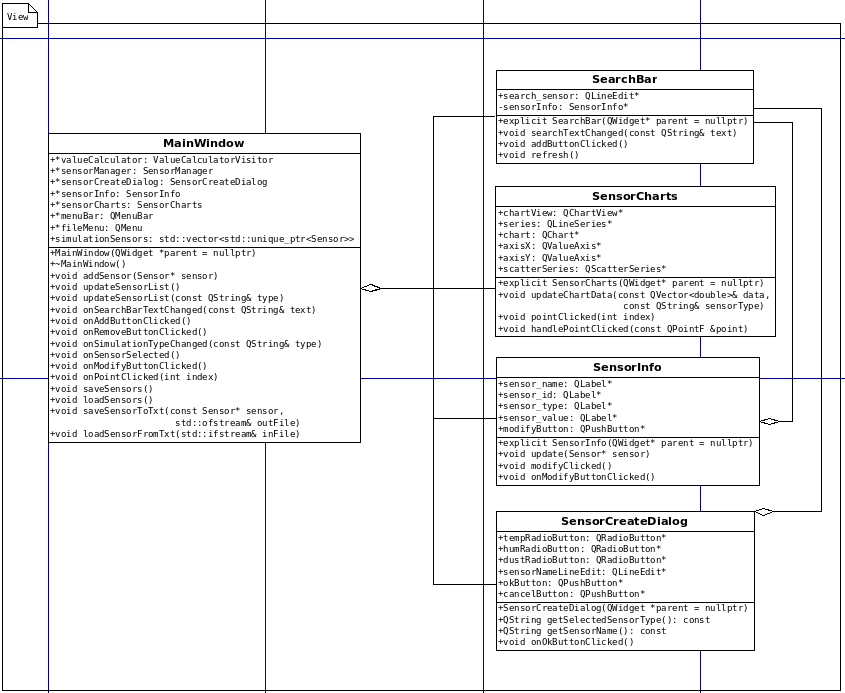
\includegraphics[width=\textwidth]{View.png}
    \caption{Parte di View}
    \label{fig:Parte di View}
\end{figure}

\section{Polimorfismo}

L’utilizzo principale del polimorfismo riguarda il design pattern Visitor nella gerarchia di Sensors. Esso viene utilizzato per estendere le funzionalità delle classi derivate senza modificare la struttura. Il calcolo del valore di ogni sensore è accessibile tramite ValueCalculatorVisitor, utilizzato quando c’è la necessità di calcolare valori differenti in base al tipo di sensore nel grafico di SensorCharts tramite la funzione calculateValue adeguata.

\section{Persistenza dei dati}
\begin{minipage}{\textwidth}
Per la persistenza dei dati viene utilizzato il formato .txt, in un unico file vengono rappresentate le informazioni principali di un Sensore, quali il Nome, l’ID, il Tipo e il Valore assegnato. Nel file .txt verrà visualizzato ogni sensore con una forma del tipo:

\begin{tabbing}
    ID: \= 10 \\
    Name: \= Sensor-10 \\
    Type: \= Humidity \\
    Value: \= 74.652 
\end{tabbing}
 Nella consegna è presente un file Sensors.txt contenente 3 sensori (uno per tipo) con le relative info.
\end{minipage}
 \section{Funzionalità implementate}

 Le funzionalità implementate sono, per semplicità, suddivise in due categorie: funzionali ed estetiche. Le prime comprendono:
 
 \begin{itemize}
    \item avvio di una simulazione del tipo di Sensore scelto
    \item conversione e salvataggio in formato TXT
    \item Modifica del nome di un Sensore
    \item Aggiunta e Rimozione di un Sensore
\end{itemize}

\noindent
Le funzionalità grafiche:

 \begin{itemize}
    \item barra dei menù in alto 
    \item utilizzo di una toolbar “File” attivabile/disattivabile (tramite menù)
    \item opzioni di Save e Open tramite toolbar File
    \item scorciatoie da tastiera per le opzioni di File (mostrate anche nelle voci del menù)
    \item scorciatoia “Ctrl+X” per la rimozione di un sensore dalla lista
    \item ogni tipologia di Sensore ha una propria disposizione in base ai valori nel Grafico
    \item utilizzo di colori per rendere più intuitivo il grafico coi suoi punti
\end{itemize}

Le funzionalità elencate sono intese in aggiunta a quanto richiesto dalle specifiche del progetto.

 \section{Rendicontazione ore}

\begin{tabular}{|c|c|c|}
    \hline
    \textbf{Attività} & \textbf{Ore Previste} & \textbf{Ore Effettive}\\
    \hline
    Studio e progettazione & 10 & 10 \\
    \hline
    Sviluppo del codice del modello & 10 & 15 \\
    \hline
    Studio del framework Qt & 10 & 15\\
    \hline
    Sviluppo del codice della GUI & 10 & 20\\
    \hline
    Test e debug & 5 & 5\\
    \hline
    Stesura della relazione & 5 & 5\\
    \hline
    \textbf{totale} & 50 & \textbf{70}\\
    \hline
\end{tabular}

\vspace{1em}

 Il monte ore è stato leggermente superato in quanto sviluppo del codice di modello e GUI ha richiesto più tempo di quanto previsto, in particolare ho riscontrato difficoltà ad implementare i metodi e le classi della parte di View, essendo Qt uno strumento totalmente nuovo per me.
\end{document}

